\documentclass{beamer}
\usepackage{graphicx}

\DeclareGraphicsExtensions{.pdf,.png,.jpg}

\mode<presentation>
{
	\usetheme{Berlin}
	\usecolortheme{default}
	\setbeamercovered{transparent}
}

\title[Optimization of Walking Parameters]
{Optimization of Walking Parameters}

\subtitle{Machine learning techniques to improve walking on bipedal robots}

\author[Girardi, Kooijman, Wiggers, Visser]{N. Girardi, C. Kooijman, A.J.Wiggers and A. Visser}

\institute[University of Amsterdam]
{
	Master Artificial Intelligence\\
	Faculty of Science (FNWI) \\
	University of Amsterdam
}

\AtBeginSection[]
{
	\begin{frame}<beamer>{Outline}
		\tableofcontents[currentsection]
	\end{frame}
}


\begin{document}


\maketitle

\begin{frame}
	\begin{center}
		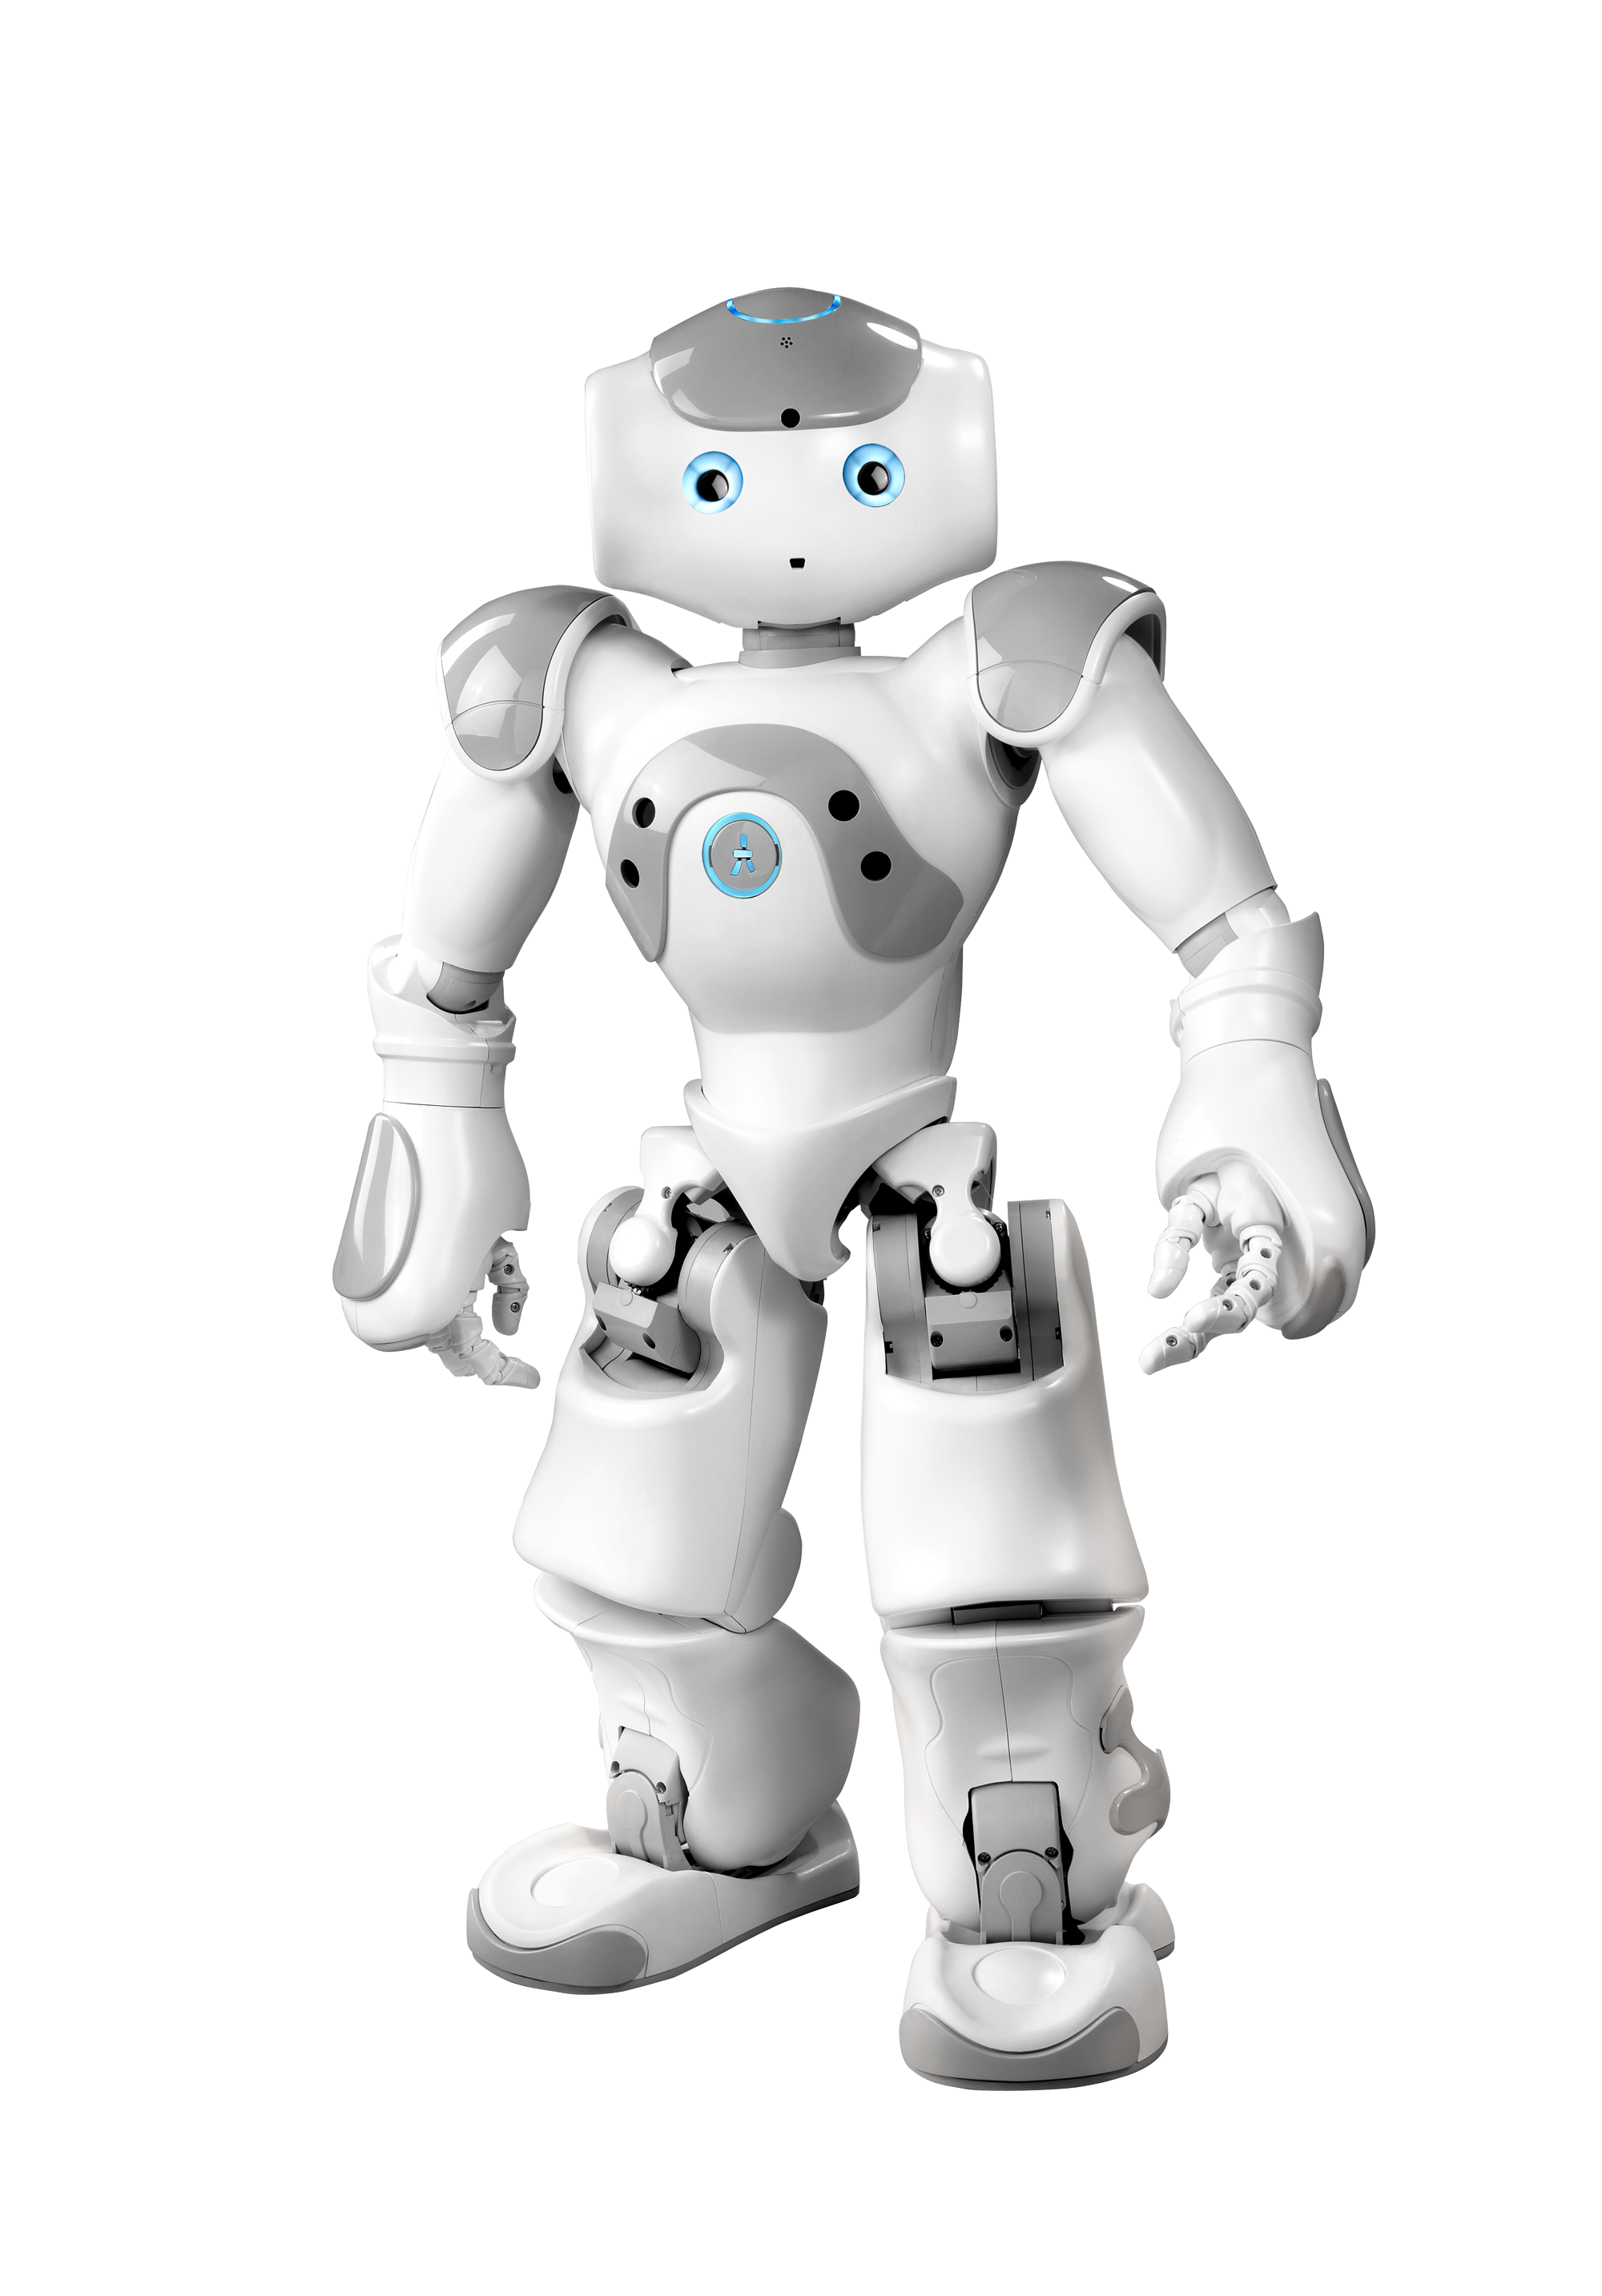
\includegraphics[height=\textheight]{NAO-4_stand}
	\end{center}
\end{frame}

\begin{frame}{Outline}
	\setcounter{tocdepth}{1}
	\tableofcontents
\end{frame}

\section{Introduction}

\subsection{Motivation}
\begin{frame}{Why RoboCup?}
	\begin{center}
		
\includegraphics[scale=.2]{robocuplogo}
	\end{center}
	\begin{itemize}
		\item Promote Robotics and AI research
		\item Make robotics appealing to the public and future generations of
			researchers
		\item Improve on state-of-the-art techniques
		\item Stimulating environment
		\item Big sharing community (especially in SPL)
	\end{itemize}
\end{frame}

\subsection{Platform}
\begin{frame}{Platform}
	\begin{center}
		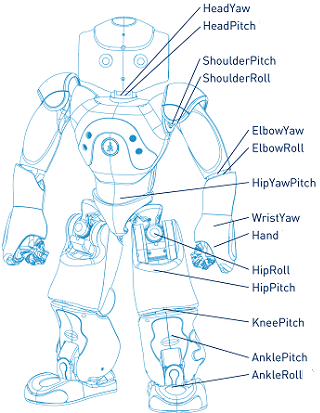
\includegraphics[width = 0.23\textwidth]{naospecsJoints}
	\end{center}
	\begin{block}{Humanoid Robot NAO}
		\begin{itemize}
			\item Nao by Aldebaran Robotics
			\item Human-like joints with 11 DOF for the legs.
		\end{itemize}
	\end{block}
\end{frame}

\section{Approach}
\begin{frame}{Framework}
% TODO IMAGE
NaoTH framework for Nao by Berlin United \cite{naothdescription}
\begin{itemize}
\item Modular: easy to extend
\item Walking engine
\item Selectable parameter set for learning
\end{itemize}
\end{frame}

\begin{frame}{Walking Engine}
	Closed loop system for walking\\
	Some parameters
	\begin{itemize}
		\item singleSupportTime
		\item stepHeight
		\item maxStep$_{x, y, \theta}$
		\item bodyOffset $x$
		\item bodyPitchOffset
		\item COMHeight
	\end{itemize}
\end{frame}		

\begin{frame}{Learning}
	Motivation:
	\begin{itemize}
		\item Difficult and time-consuming to design by hand
		\item Increasing error due to servo heat
		\item Robots age
		\item Hot research topic
		\item Not limited to Nao
	\end{itemize}
\end{frame}

\subsection{Genetic Algorithm}
\begin{frame}{Genetic Algorithm}
	Similar to biology: Survival of the fittest.
    \begin{itemize}
		\item Transmission
		\item Crossover
		\item Mutation
	\end{itemize}


    Parameters
	\begin{itemize}
		\item Population size 
		\item Number of parents
		\item Survivors
	\end{itemize}
\end{frame}

\begin{frame}{Fitness}
    Evaluation tasks representative for real game:
    \begin{itemize}
        \item Walking forward/backward
		\item Strafing
	    \item Go to point
		\item Rapid change of direction
		\item Combinations
    \end{itemize}

    Extra:
    \begin{itemize}
    \item Penalize falling down.    
    \item Fitness based on walking distance.
    \end{itemize}
\end{frame}

\begin{frame}
	\begin{itemize}
		\item Gui for SimSpark (official simulator) or real world evaluation
	\end{itemize}
	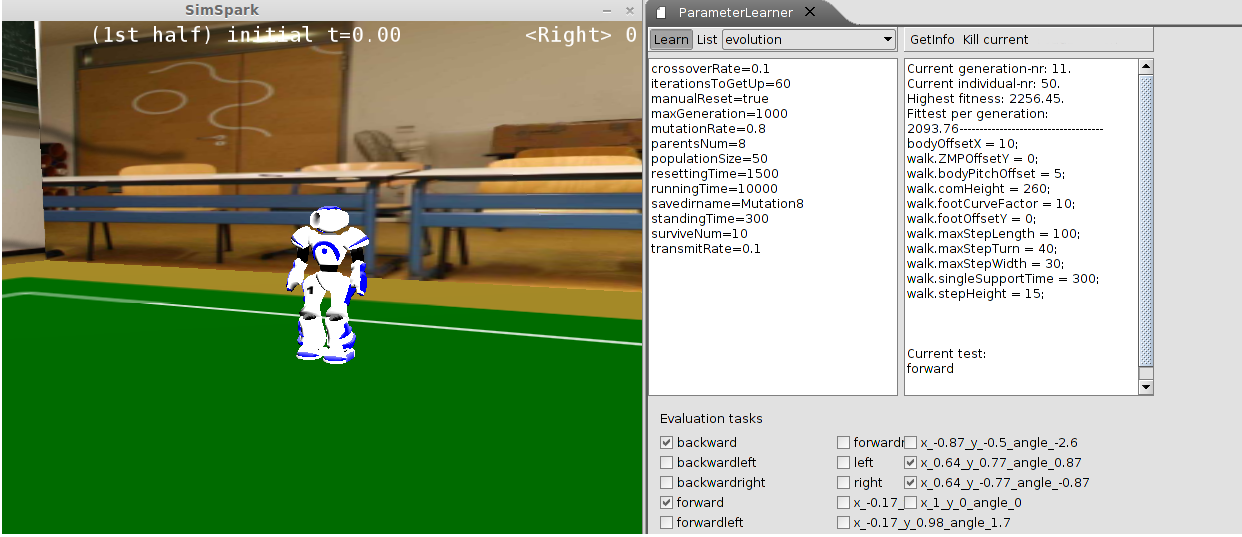
\includegraphics[width=\textwidth]{GUI}
\end{frame}

\section{Results}
\begin{frame}{Results}
	\begin{center}
		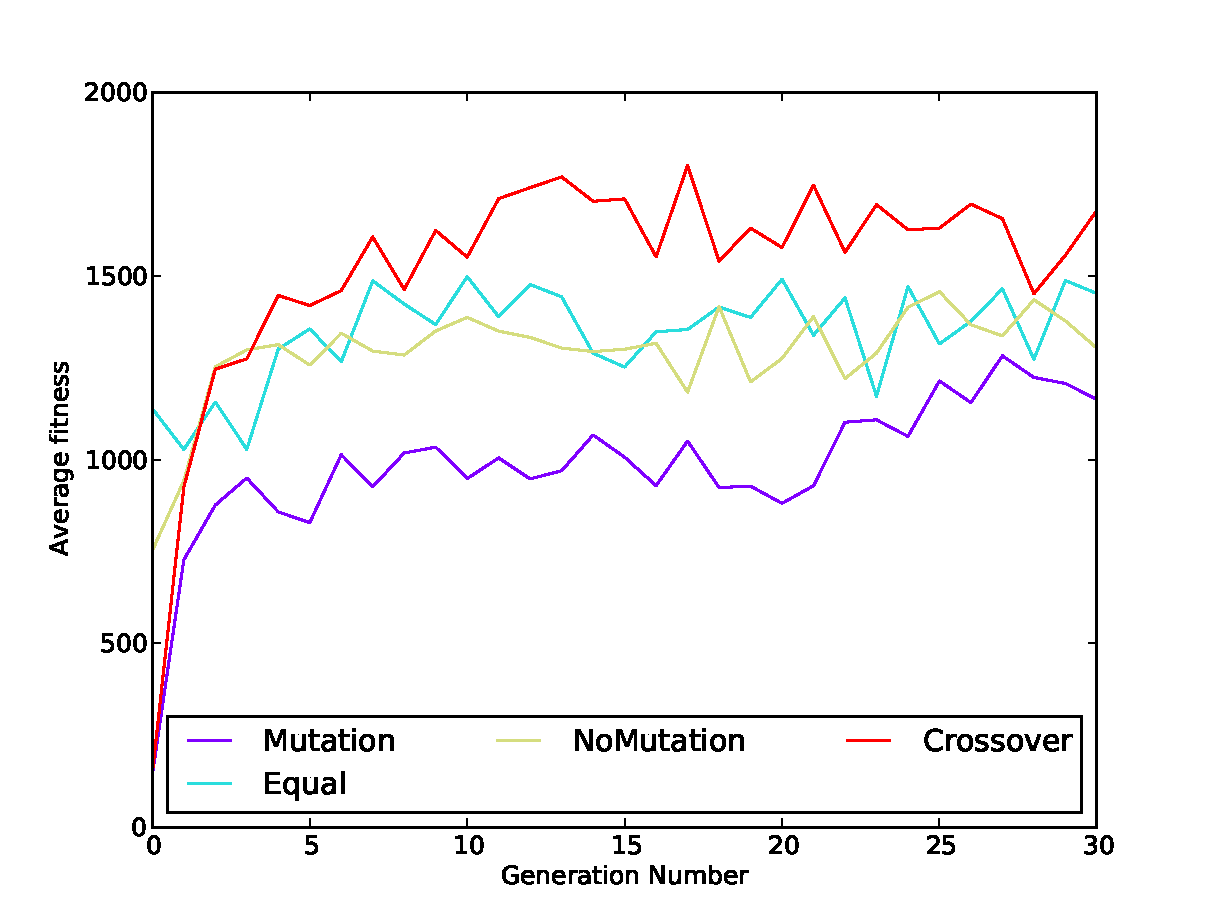
\includegraphics[width=.5\textwidth]{relevant_avg}
	\end{center}
\begin{itemize}
	\item Fitness increases for first 10-15 generations in simulation
	\item Success in simulation does not (yet) translate to real world
\end{itemize}
\end{frame}

\section{Future work}
\begin{frame}{Future work}
\begin{itemize}
\item Real-time parameter adjustment
\item Different parameters for different motions
\item On-line learning
	\begin{itemize}
		\item Evaluation during matches
	\end{itemize}
\item Multi-objective (e.g. speed, stability, manoeuvrability, etc.)
\end{itemize}
\end{frame}

\begin{frame}{On-line Learning}
\begin{itemize}
\item More time to learn (robots need to `rest')
\item Best representation of real game
\item Can account for changing conditions (overheating)
\item Individual robots are different
\end{itemize}
\end{frame}

\section{Questions}

\begin{frame}{Questions}
	Questions?
\end{frame}

\begin{frame}{References}
	\bibliographystyle{apalike}
	\bibliography{pres}
\end{frame}

\end{document}
% vim: set spell : spelllang=en_gb :

